\chapter{Statistique de la mesure chimique}\label{ch:b2:measurement-statistics}

Deux laboratoires mesurent le plomb d'une même eau du robinet et trouvent 9.6 et \qty{11.2}{\micro g/L}.
La valeur guide pour l'eau de boisson est de \qty{10}{\micro g/L}. Cette eau est-elle potable~? Les deux
laboratoires sont-ils même en désaccord, ou les deux résultats sont-ils une même valeur vue à travers la
dispersion de deux mesures~? Un nombre issu d'une analyse ne signifie rien sans son incertitude, et ce
chapitre donne les outils pour la calculer~: la statistique des mesures répétées, la propagation des
incertitudes dans un calcul, l'étalonnage par les moindres carrés, et les limites au-dessous desquelles
une méthode ne voit plus rien.
% ledger: who:lead

\begin{omfigure}
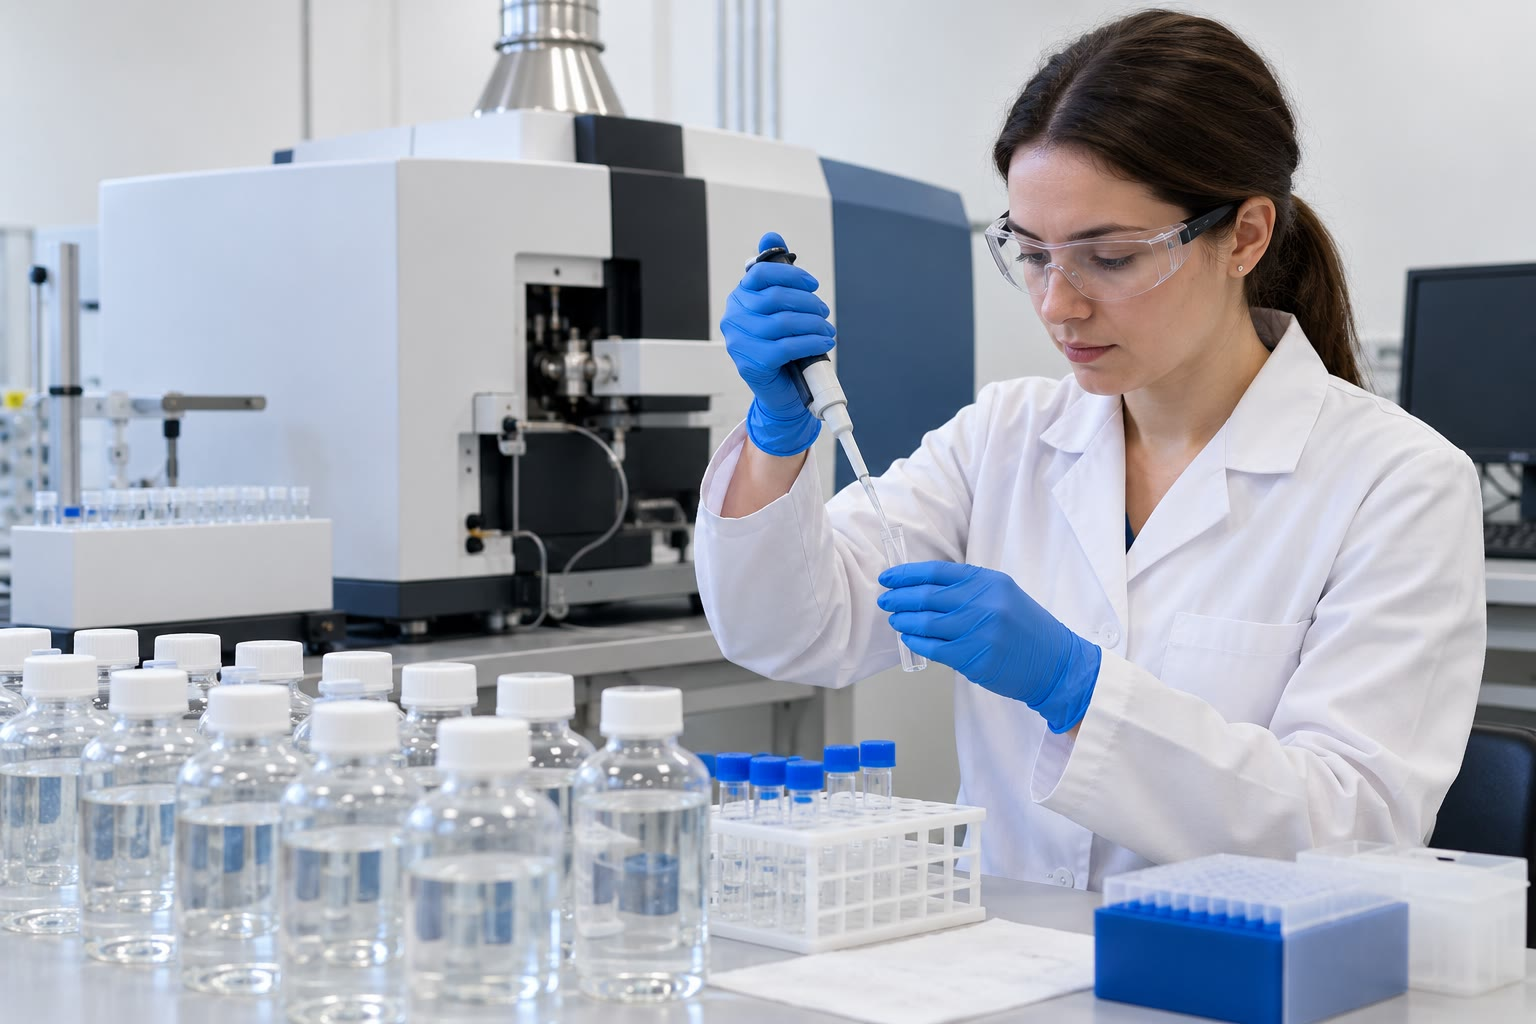
\includegraphics[width=0.56\linewidth]{images/book3/ai/b2-34-water-lab.jpg}

{\small Un laboratoire d'analyse des eaux~: flacons d'échantillons, une technicienne qui pipette, un
analyseur élémentaire à l'arrière-plan (illustration).}
\end{omfigure}

\begin{recall}
Le volume de première année~: incertitude de mesure, incertitude-type, évaluations de type A et de type B,
incertitude élargie, incertitude relative, écart normalisé $z$ entre deux valeurs, et la promesse d'une
démonstration de $u(\bar x) = s/\sqrt n$ et d'une règle générale de propagation. Le volume scolaire~: la
droite d'étalonnage. \Cref{ch:b2:mass-spec-atomic}~: l'absorption atomique.
\end{recall}

\section{Mesures répétées}

Répétons une mesure~: les résultats se dispersent. On traite chaque résultat $x_i$ comme une variable
aléatoire de moyenne $\mu$ (la valeur que la méthode donnerait en moyenne) et d'écart type $\sigma$~;
quand de nombreuses petites causes indépendantes s'additionnent, les résultats suivent la loi normale
(gaussienne), environ 68~\% d'entre eux se situant dans $\mu \pm \sigma$ et 95~\% dans $\mu \pm 1.96\sigma$.

\begin{definition}[Dispersion]\label{def:b2:measurement-statistics:dispersion}
Pour $n$ résultats $x_1, \dots, x_n$ de moyenne $\bar x$, l'\emph{écart type
expérimental}\index{ecart type experimental@écart type expérimental} vaut $s = \sqrt{\sum (x_i - \bar x)^2/(n-1)}$~;
il estime $\sigma$. L'\emph{écart type de la moyenne}\index{ecart type de la moyenne@écart type de la moyenne} est
l'écart type de $\bar x$ sur de nombreuses séries de $n$ résultats, estimé par $s/\sqrt n$.
\end{definition}

Le diviseur $n - 1$ plutôt que $n$ corrige le fait que les écarts sont pris par rapport à $\bar x$,
lui-même calculé à partir des mêmes données, ce qui les rend légèrement trop petits~: $n - 1$ est le
nombre d'écarts indépendants, le nombre de degrés de liberté.

\begin{theorem}[Variance de la moyenne]\label{thm:b2:measurement-statistics:mean-variance}
Si $x_1, \dots, x_n$ sont indépendants, chacun de variance $\sigma^2$, alors $\operatorname{var}(\bar x) =
\sigma^2/n$~: l'\omterm{def:b2:measurement-statistics:dispersion}{écart type de la moyenne} vaut $\sigma/\sqrt n$.
\end{theorem}

\begin{proof}
Pour des variables indépendantes, la variance d'une somme est la somme des variances, et
$\operatorname{var}(cX) = c^2\operatorname{var}(X)$. Ainsi $\operatorname{var}(\bar x) =
\operatorname{var}\bigl(\tfrac1n\sum x_i\bigr) = \tfrac{1}{n^2}\sum\operatorname{var}(x_i) =
\tfrac{1}{n^2}\,n\sigma^2 = \sigma^2/n$. Remplacer $\sigma$ par son estimation $s$ donne l'incertitude-type
de type A $u(\bar x) = s/\sqrt n$ admise dans le volume de première année.
\end{proof}

\section{Intervalles de confiance}

\begin{definition}[Intervalle de confiance]\label{def:b2:measurement-statistics:confidence}
Un \emph{intervalle de confiance}\index{intervalle de confiance} au \emph{niveau de confiance}\index{niveau de confiance}
$1 - \alpha$ (souvent 95~\%) est un intervalle calculé à partir des données selon une règle qui,
appliquée à de nombreuses séries, contient la valeur vraie dans une fraction $1 - \alpha$ d'entre elles.
Pour la moyenne de $n$ résultats, il vaut $\bar x \pm t\,s/\sqrt n$, où $t$ est le \emph{coefficient de
Student}\index{coefficient de Student} pour $n - 1$ degrés de liberté et ce niveau.
\end{definition}

\begin{proposition}[Loi de Student]\label{prop:b2:measurement-statistics:student}
Pour $n$ résultats normaux indépendants, $T = (\bar x - \mu)/(s/\sqrt n)$ suit la loi de Student à
$n - 1$ degrés de liberté, dont la densité est proportionnelle à $(1 + t^2/\nu)^{-(\nu+1)/2}$ avec
$\nu = n - 1$. Elle est plus large que la loi normale et tend vers elle quand $n$ augmente.
\end{proposition}

\admitted

Diviser par $s$ au lieu du $\sigma$ inconnu ajoute la dispersion de $s$ elle-même, grande quand $n$ est
petit~; d'où des queues plus lourdes, et des coefficients supérieurs à 1.96. Le tableau donne les
coefficients à 95~\%, calculés à partir de la densité.

\begin{omfigure}
\begin{minipage}[c]{0.56\linewidth}
\begin{tikzpicture}
\begin{axis}[width=\linewidth, height=4.8cm, xmin=-5, xmax=5, ymin=0, ymax=0.43,
  xlabel={$t$}, ylabel={densité}, label style={font=\small}, tick label style={font=\scriptsize},
  legend style={font=\scriptsize, at={(0.98,0.98)}, anchor=north east}, legend cell align=left]
\addplot[omThm, thick] table[x=t, y=nu2] {figdata/out/bachelor-2-regression-c.dat};
\addplot[omMeth, thick] table[x=t, y=nu5] {figdata/out/bachelor-2-regression-c.dat};
\addplot[black, thick, dashed] table[x=t, y=normal] {figdata/out/bachelor-2-regression-c.dat};
\legend{$\nu = 2$, $\nu = 5$, loi normale}
\end{axis}
\end{tikzpicture}
\end{minipage}\hfill
\begin{minipage}[c]{0.4\linewidth}\centering
\small
\begin{tabular}{rr}
\hline
$\nu = n - 1$ & $t$ (95~\%) \\
\hline
1 & 12.706 \\
2 & 4.303 \\
3 & 3.182 \\
4 & 2.776 \\
5 & 2.571 \\
9 & 2.262 \\
20 & 2.086 \\
$\infty$ & 1.960 \\
\hline
\end{tabular}
\end{minipage}
\par\vspace{4pt}

{\small Densités de Student à 2 et 5 degrés de liberté comparées à la loi normale, et coefficients
bilatéraux à 95~\%, calculés par intégration de la densité (la dernière ligne correspond à la loi normale).}
% figdata: bachelor-2/regression.py parts c, e
\end{omfigure}

\begin{method}[Un intervalle de confiance pour une moyenne]\label{met:b2:measurement-statistics:confidence-interval}
\begin{enumerate}
  \item Calculer $\bar x$ et $s$ des $n$ résultats~; vérifier qu'aucun résultat n'est grossièrement aberrant.
  \item Lire $t$ pour $\nu = n - 1$ au niveau choisi.
  \item Donner $\bar x \pm t\,s/\sqrt n$, l'incertitude étant arrondie à un ou deux chiffres significatifs
        et la moyenne à la même décimale.
  \item Pour comparer à une valeur de référence $x_{\mathrm{ref}}$, calculer $|\bar x - x_{\mathrm{ref}}|/(s/\sqrt
        n)$~: au-dessus de $t$, l'écart est significatif à ce niveau~; au-dessous, les données ne mettent
        pas en évidence d'écart (ce qui ne prouve pas qu'il n'y en a pas).
\end{enumerate}
\end{method}

\section{Propagation des incertitudes}

\begin{theorem}[Loi de propagation des incertitudes]\label{thm:b2:measurement-statistics:propagation}
Si $y = f(x_1, \dots, x_n)$, où les $x_i$ sont indépendants, d'incertitudes-types $u(x_i)$ assez
petites pour que $f$ soit presque linéaire sur leur étendue, alors
\begin{equation*}
u^2(y) = \sum_{i=1}^{n}\left(\frac{\partial f}{\partial x_i}\right)^2 u^2(x_i).
\end{equation*}
\end{theorem}

\begin{proof}
Au premier ordre (Taylor), $y - f(\mu_1, \dots, \mu_n) \approx \sum c_i(x_i - \mu_i)$ avec $c_i = \partial
f/\partial x_i$ aux moyennes. La variance d'une combinaison linéaire de variables indépendantes vaut
$\sum c_i^2\operatorname{var}(x_i)$ (comme au \cref{thm:b2:measurement-statistics:mean-variance})~; avec
$\operatorname{var}(x_i) = u^2(x_i)$, c'est le résultat.
\end{proof}

\begin{corollary}[Sommes et produits]\label{cor:b2:measurement-statistics:products}
Pour une somme ou une différence, les incertitudes-types s'ajoutent quadratiquement~: $u^2(x_1 \pm x_2) = u^2(x_1) +
u^2(x_2)$. Pour un produit ou un quotient $y = x_1^{a}x_2^{b}\cdots$, les incertitudes relatives s'ajoutent
quadratiquement, chacune pondérée par son exposant~: $\bigl(u(y)/y\bigr)^2 = a^2\bigl(u(x_1)/x_1\bigr)^2 +
b^2\bigl(u(x_2)/x_2\bigr)^2 + \cdots$
\end{corollary}

\begin{proof}
Pour une somme, les dérivées partielles valent $\pm1$. Pour $y = x_1^ax_2^b$, $\partial y/\partial x_1 =
a\,y/x_1$ et $\partial y/\partial x_2 = b\,y/x_2$~; le théorème donne $u^2(y) = a^2y^2u^2(x_1)/x_1^2 +
b^2y^2u^2(x_2)/x_2^2$~; diviser par $y^2$.
\end{proof}

\begin{method}[Propager]\label{met:b2:measurement-statistics:propagate}
\begin{enumerate}
  \item Écrire le résultat comme une formule des grandeurs mesurées~; énumérer chaque entrée avec son
        incertitude-type (type A ou B).
  \item Pour les produits et les quotients, travailler avec les incertitudes relatives~; pour les sommes,
        avec les incertitudes absolues~; sinon, prendre les dérivées partielles.
  \item Combiner quadratiquement~; repérer le terme dominant~: améliorer les autres est un effort perdu.
  \item Multiplier par le facteur d'élargissement (2, ou le $t$ de Student quand le terme dominant vient
        de peu de répétitions) pour obtenir une incertitude élargie.
\end{enumerate}
\end{method}

\section{Étalonnage}

\begin{definition}[Courbe d'étalonnage]\label{def:b2:measurement-statistics:calibration}
Une \emph{courbe d'étalonnage}\index{courbe d'etalonnage@courbe d'étalonnage} relie le signal $y$ d'un
instrument à la concentration $x$, à partir d'étalons de concentration connue. La \emph{droite des
moindres carrés}\index{droite des moindres carres@droite des moindres carrés} $y = a + bx$ est la droite qui minimise $S = \sum (y_i - a -
bx_i)^2$~; chaque $e_i = y_i - a - bx_i$ est un \emph{résidu}\index{residu@résidu}.
\end{definition}

\begin{theorem}[Droite des moindres carrés]\label{thm:b2:measurement-statistics:least-squares}
Avec $\bar x$, $\bar y$ les moyennes, $S_{xx} = \sum(x_i - \bar x)^2$ et $S_{xy} = \sum(x_i - \bar x)(y_i -
\bar y)$, la \omterm{def:b2:measurement-statistics:calibration}{droite des moindres carrés} a pour coefficients
\begin{equation*}
b = \frac{S_{xy}}{S_{xx}}, \qquad a = \bar y - b\bar x.
\end{equation*}
\end{theorem}

\begin{proof}
$S$ est une fonction quadratique de $a$ et $b$. Ses dérivées partielles s'annulent au minimum~:
$\partial S/\partial a = -2\sum(y_i - a - bx_i) = 0$ donne $a = \bar y - b\bar x$~; en reportant dans
$\partial S/\partial b = -2\sum x_i(y_i - a - bx_i) = 0$, on obtient $\sum x_i\bigl((y_i - \bar y) - b(x_i -
\bar x)\bigr) = 0$, c'est-à-dire $S_{xy} = bS_{xx}$ (car $\sum \bar x(y_i - \bar y) = \sum \bar x(x_i - \bar
x) = 0$). Les dérivées secondes forment la matrice
\[\begin{pmatrix} 2n & 2\sum x_i\\ 2\sum x_i & 2\sum x_i^2\end{pmatrix},\]
dont la diagonale est positive et dont le déterminant $4nS_{xx}$ est positif quand les $x_i$ ne sont pas
tous égaux~: le point stationnaire est un minimum.
\end{proof}

\begin{proposition}[Lecture d'une concentration]\label{prop:b2:measurement-statistics:interpolation}
Pour $n$ étalons d'écart type résiduel $s_{y/x} = \sqrt{\sum e_i^2/(n-2)}$, un échantillon lu
$m$ fois avec un signal moyen $\bar y_0$ a pour concentration $x_0 = (\bar y_0 - a)/b$, d'écart type
\begin{equation*}
s_{x_0} = \frac{s_{y/x}}{b}\sqrt{\frac1m + \frac1n + \frac{(\bar y_0 - \bar y)^2}{b^2S_{xx}}},
\end{equation*}
à utiliser avec le $t$ de Student pour $n - 2$ degrés de liberté.
\end{proposition}

\admitted

Les trois termes sous la racine sont la dispersion des lectures de l'échantillon, l'incertitude sur la
hauteur de la droite et celle sur sa pente~; la dernière s'annule au centre du domaine d'étalonnage, là
où il vaut mieux lire les échantillons.

\begin{omfigure}
\begin{tikzpicture}
\begin{axis}[width=0.5\linewidth, height=5cm, xmin=-1, xmax=22, ymin=0, ymax=0.22,
  xlabel={plomb (\unit{\micro g/L})}, ylabel={absorbance}, label style={font=\small},
  tick label style={font=\scriptsize}, scaled y ticks=false,
  yticklabel style={/pgf/number format/fixed, /pgf/number format/precision=2}]
\addplot[omDef, thick] table[x=x, y=line] {figdata/out/bachelor-2-regression-b.dat};
\addplot[only marks, mark=*, mark size=1.8pt, omThm] table[x=x, y=A] {figdata/out/bachelor-2-regression-a.dat};
\end{axis}
\end{tikzpicture}\hfill
\begin{tikzpicture}
\begin{axis}[width=0.5\linewidth, height=5cm, xmin=-1, xmax=22, ymin=-0.002, ymax=0.002,
  xlabel={plomb (\unit{\micro g/L})}, ylabel={résidu}, label style={font=\small},
  tick label style={font=\scriptsize}, scaled y ticks=false, ycomb,
  yticklabel style={/pgf/number format/fixed, /pgf/number format/precision=3},
  extra y ticks={0}, extra y tick style={grid=major, grid style={black!50}}]
\addplot[omThm, thick, mark=*, mark size=1.6pt] table[x=x, y=res] {figdata/out/bachelor-2-regression-a.dat};
\end{axis}
\end{tikzpicture}

{\small Étalonnage du plomb par absorption atomique en four graphite à \qty{283.3}{nm} (données de
l'exercice, reprises dans le problème). À gauche~: les cinq étalons et la \omterm{def:b2:measurement-statistics:calibration}{droite des moindres carrés}. À
droite~: les \omterm{def:b2:measurement-statistics:calibration}{résidus}, petits et sans structure~: une droite convient.}
% figdata: bachelor-2/regression.py parts a, b
% ledger: asd:Pb283
\end{omfigure}

\begin{method}[Étalonner]\label{met:b2:measurement-statistics:calibrate}
\begin{enumerate}
  \item Préparer cinq étalons ou plus couvrant le domaine attendu, dans la même matrice que les
        échantillons, ainsi qu'un blanc.
  \item Ajuster la \omterm{def:b2:measurement-statistics:calibration}{droite des moindres carrés}~; tracer les \omterm{def:b2:measurement-statistics:calibration}{résidus}. Une structure courbe signifie que la
        réponse n'est pas linéaire~: réduire le domaine ou ajuster une courbe. Un \omterm{def:b2:measurement-statistics:calibration}{résidu} isolé important
        désigne un étalon défectueux.
  \item Lire les échantillons, de préférence vers le milieu du domaine, en plusieurs répétitions~;
        calculer $x_0$ et
        $s_{x_0}$.
  \item Donner $x_0 \pm t\,s_{x_0}$ après correction de chaque dilution, en ajoutant l'incertitude propagée
        de la dilution si elle n'est pas négligeable.
\end{enumerate}
\end{method}

\begin{definition}[Ajouts dosés]\label{def:b2:measurement-statistics:standard-addition}
Dans la \emph{méthode des ajouts dosés}\index{methode des ajouts doses@méthode des ajouts dosés}, on
ajoute des quantités connues d'analyte à des parts égales de l'échantillon lui-même~; on trace le signal
en fonction de la concentration ajoutée, et la concentration de l'analyte dans l'échantillon est la
distance entre l'origine et le point où la droite, extrapolée jusqu'au signal nul, coupe l'axe, $a/b$.
\end{definition}

\begin{method}[Ajouts dosés]\label{met:b2:measurement-statistics:standard-addition}
\begin{enumerate}
  \item L'utiliser quand la matrice de l'échantillon modifie la réponse (sels, acides, matière organique),
        si bien que des étalons dans l'eau pure donneraient une pente erronée.
  \item Doper des parts égales par des quantités connues croissantes, compléter toutes au même volume,
        mesurer.
  \item Ajuster la droite~; la concentration dans les solutions mesurées vaut $a/b$~; corriger de la dilution.
  \item La réponse doit être linéaire dès zéro~: vérifier les \omterm{def:b2:measurement-statistics:calibration}{résidus}.
\end{enumerate}
\end{method}

\begin{omfigure}
\begin{tikzpicture}
\begin{axis}[width=0.62\linewidth, height=5cm, xmin=-4, xmax=7, ymin=0, ymax=0.42,
  xlabel={concentration ajoutée (\unit{mg/L})}, ylabel={absorbance}, label style={font=\small},
  tick label style={font=\scriptsize}, axis lines=left, scaled y ticks=false,
  yticklabel style={/pgf/number format/fixed, /pgf/number format/precision=1}]
\draw[black!40] (axis cs:0,0) -- (axis cs:0,0.42);
\addplot[omDef, thick, densely dashed] table[x=x, y=line] {figdata/out/bachelor-2-regression-d-line.dat};
\addplot[only marks, mark=*, mark size=1.8pt, omThm] table[x=x, y=A] {figdata/out/bachelor-2-regression-d.dat};
\draw[<->, omMeth, thick] (axis cs:-3.11,0.06) -- (axis cs:0,0.06); \node[omMeth, below, font=\scriptsize] at (axis cs:-0.8,0.055) {$a/b$};
\end{axis}
\end{tikzpicture}

{\small Ajouts dosés (données de l'exercice)~: absorbance d'un échantillon dopé par 0, 2, 4 et
\qty{6}{mg/L} d'analyte. La droite atteint le signal nul à \qty{-3.11}{mg/L}~: la solution mesurée
contenait \qty{3.11}{mg/L}.}
% figdata: bachelor-2/regression.py part d
\end{omfigure}

\section{Détection, quantification et validation}

\begin{definition}[Limites]\label{def:b2:measurement-statistics:limits}
La \emph{limite de détection}\index{limite de detection@limite de détection} d'une méthode est la plus
petite concentration dont le signal peut être distingué de celui d'un blanc avec un faible risque donné
de fausse détection~; la \emph{limite de quantification}\index{limite de quantification} est la plus
petite concentration qui peut être mesurée avec une incertitude relative acceptable.
\end{definition}

\begin{proposition}[Estimations usuelles]\label{prop:b2:measurement-statistics:lod}
Avec $s_{\mathrm{blanc}}$ l'écart type de signaux de blanc répétés et $b$ la pente de la droite
d'étalonnage, $x_{\mathrm{LD}} \approx 3s_{\mathrm{blanc}}/b$ et $x_{\mathrm{LQ}} \approx
10s_{\mathrm{blanc}}/b$.
\end{proposition}

\begin{proof}[Argument]
Si les signaux de blanc sont normaux d'écart type $s_{\mathrm{blanc}}$, un blanc dépasse sa moyenne de
plus de $3s_{\mathrm{blanc}}$ avec une probabilité d'environ 0.13~\% (queue unilatérale de la loi normale
au-delà de 3 écarts types)~: déclarer «~détecté~» un signal au-dessus de ce seuil confond rarement un
blanc avec un échantillon. Un signal situé $10s_{\mathrm{blanc}}$ au-dessus du blanc a un écart type relatif
d'environ 10~\%, le seuil habituel d'un résultat quantitatif. Diviser par $b$ convertit les signaux en
concentrations.
\end{proof}

\begin{definition}[Validation]\label{def:b2:measurement-statistics:validation}
La \emph{justesse}\index{justesse} est l'étroitesse de l'accord entre la moyenne d'un grand nombre de
résultats et la valeur vraie~; leur différence est le \emph{biais}\index{biais}. La \emph{fidélité}\index{fidelite@fidélité}
est l'étroitesse de l'accord entre des résultats indépendants, exprimée par un écart type~: la
\emph{répétabilité}\index{repetabilite@répétabilité} dans les mêmes conditions (même opérateur, même
instrument, même laboratoire, court intervalle de temps), la \emph{reproductibilité}\index{reproductibilite@reproductibilité}
dans des conditions modifiées (laboratoires différents). La \emph{validation de méthode}\index{validation de methode@validation de méthode}
est l'ensemble des expériences qui établissent, pour une méthode, sa justesse, sa fidélité, sa linéarité
et son domaine, et ses \omterm{def:b2:measurement-statistics:limits}{limites de détection} et de quantification.
\end{definition}

La \omterm{def:b2:measurement-statistics:validation}{justesse} se vérifie à l'aide d'un matériau de référence certifié ou par dopage~; la \omterm{def:b2:measurement-statistics:validation}{fidélité} par des
répétitions dans un même laboratoire et par des comparaisons entre laboratoires. Une méthode peut être
fidèle mais biaisée, chaque résultat proche des autres et tous faux~: la \omterm{def:b2:measurement-statistics:validation}{fidélité} ne prouve pas la \omterm{def:b2:measurement-statistics:validation}{justesse}.

\begin{history}[Student, 1908]
\begin{minipage}[t]{0.17\linewidth}
\vspace{0pt}
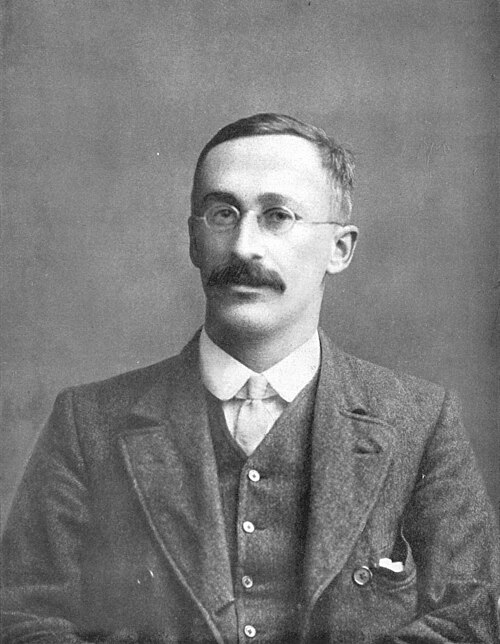
\includegraphics[width=\linewidth]{images/book3/gosset.jpg}
\end{minipage}\hfill
\begin{minipage}[t]{0.79\linewidth}
\vspace{0pt}
William Sealy Gosset, chimiste au service d'une brasserie, devait juger des matières premières à partir
de très peu d'échantillons, bien trop peu pour la loi normale. En 1908, il publia la loi de la moyenne
divisée par l'écart type de l'échantillon, sous le pseudonyme «~Student~», parce que son employeur
n'autorisait pas son personnel à publier sous son nom. La loi de Student sert chaque fois qu'un analyste
donne un intervalle à partir de trois ou quatre répétitions. (Photographie, 1908~: domaine public~;
Wikimedia Commons.)
\end{minipage}
\end{history}

\section{Exercices}

\begin{exercise}[$\star$]\label{exo:b2:measurement-statistics:1}
Cinq titrages donnent 12.45, 12.50, 12.48, 12.52 et \qty{12.46}{mL}. Calculer la moyenne, l'\omterm{def:b2:measurement-statistics:dispersion}{écart type
expérimental} et l'\omterm{def:b2:measurement-statistics:dispersion}{écart type de la moyenne}.
\end{exercise}

\begin{exercise}[$\star$]\label{exo:b2:measurement-statistics:2}
Donner l'\omterm{def:b2:measurement-statistics:confidence}{intervalle de confiance} à 95~\% de la moyenne de l'exercice~1.
\end{exercise}

\begin{exercise}[$\star$]\label{exo:b2:measurement-statistics:3}
On prépare une solution en dissolvant $m = \qty{0.5000}{g}$ ($u = \qty{0.0002}{g}$) d'un solide dans une
fiole de
$V = \qty{250.0}{mL}$ ($u = \qty{0.15}{mL}$). Calculer l'incertitude-type relative de $c = m/(MV)$,
la masse molaire étant connue avec assez d'exactitude.
\end{exercise}

\begin{exercise}[$\star$]\label{exo:b2:measurement-statistics:4}
Ajuster la \omterm{def:b2:measurement-statistics:calibration}{droite des moindres carrés} passant au mieux par $(0, 0.02)$, $(1, 0.21)$, $(2, 0.39)$, $(3, 0.62)$.
\end{exercise}

\begin{exercise}[$\star\star$]\label{exo:b2:measurement-statistics:5}
Une solution de référence certifiée contient \qty{10.00}{mg/L} d'un élément. Cinq analyses donnent une
moyenne de
\qty{10.12}{mg/L} avec $s = \qty{0.08}{mg/L}$. La méthode est-elle biaisée au niveau de 95~\%~?
\end{exercise}

\begin{exercise}[$\star\star$]\label{exo:b2:measurement-statistics:6}
Une concentration en ions oxonium est connue avec une incertitude-type relative de 2~\%. Quelle est
l'incertitude-type du pH~?
\end{exercise}

\begin{exercise}[$\star\star$]\label{exo:b2:measurement-statistics:7}
Dix blancs ont $s = 0.0012$ unité d'absorbance~; la pente d'étalonnage vaut \qty{0.0098}{L/\micro g}.
Estimer les \omterm{def:b2:measurement-statistics:limits}{limites de détection} et de quantification.
\end{exercise}

\begin{exercise}[$\star\star$]\label{exo:b2:measurement-statistics:8}
Dans l'expérience d'ajouts dosés de la figure, les quatre parts avaient été préparées en diluant
\qty{10.0}{mL} d'échantillon jusqu'à \qty{50.0}{mL}. Donner la concentration dans l'échantillon.
\end{exercise}

\begin{exercise}[$\star\star$]\label{exo:b2:measurement-statistics:9}
Dans une étude interlaboratoires, chaque laboratoire obtient $s = \qty{0.05}{mg/L}$ sur ses propres
répétitions, mais les résultats des différents laboratoires se dispersent avec $s = \qty{0.15}{mg/L}$.
Nommer les deux grandeurs et expliquer la différence.
\end{exercise}

\begin{exercise}[$\star\star\star$]\label{exo:b2:measurement-statistics:10}
Montrer que la \omterm{def:b2:measurement-statistics:calibration}{droite des moindres carrés} passe par $(\bar x, \bar y)$ et que la somme de ses \omterm{def:b2:measurement-statistics:calibration}{résidus} est nulle.
\end{exercise}

\begin{exercise}[$\star\star\star$]\label{exo:b2:measurement-statistics:11}
Une solution mère est diluée cent fois, soit en une étape (\qty{1.000}{mL} dans \qty{100.0}{mL}), soit
en deux étapes au dixième (\qty{10.00}{mL} dans \qty{100.0}{mL}, deux fois). Incertitudes-types~: pipette
de 1 mL, \qty{0.006}{mL}~; pipette de 10 mL, \qty{0.02}{mL}~; fiole de 100 mL, \qty{0.08}{mL} (données de
l'exercice). Quelle voie est la plus précise~?
\end{exercise}

\begin{exercise}[$\star\star\star$]\label{exo:b2:measurement-statistics:12}
Les deux laboratoires de l'introduction trouvent 9.6 et \qty{11.2}{\micro g/L} avec des incertitudes-types
de 0.4 et \qty{0.5}{\micro g/L} (données de l'exercice). Leurs résultats sont-ils compatibles~? Que dit
chacun d'eux de la valeur guide~?
\end{exercise}

\section{Problème~: le plomb dans l'eau du robinet}

\begin{problem}[{Problème du week-end --- un étalonnage d'absorption atomique par les moindres carrés,
la concentration d'un échantillon avec son intervalle de confiance, la dilution et les limites, et un
verdict au regard de la valeur guide}]
\label{pb:b2:measurement-statistics:1}
Données de l'exercice. Le plomb est mesuré par absorption atomique en four graphite à \qty{283.3}{nm}.
Étalons (\unit{\micro g/L}~; absorbance)~: 0.0~; 0.003, 5.0~; 0.051, 10.0~; 0.101, 15.0~; 0.148, 20.0~;
0.199. L'eau du robinet (\qty{50.0}{mL}) est acidifiée par \qty{0.50}{mL} d'acide nitrique~; trois
lectures de cette solution donnent 0.104, 0.098 et 0.101. Dix blancs~: 0.002, 0.004, 0.003, 0.001,
0.003, 0.005, 0.002, 0.003, 0.004, 0.003. Incertitudes-types des volumes~: \qty{0.03}{mL} pour 50.0 mL,
\qty{0.005}{mL} pour 0.50 mL. Valeur guide~: \qty{10}{\micro g/L}.
% ledger: who:lead, asd:Pb283

\medskip
\noindent\textbf{Partie I --- Étalonnage.}
\begin{enumerate}
  \item Pourquoi les étalons sont-ils préparés dans le même acide nitrique que les échantillons~?
  \item Calculer la pente et l'ordonnée à l'origine de la \omterm{def:b2:measurement-statistics:calibration}{droite des moindres carrés}.
  \item Calculer les cinq \omterm{def:b2:measurement-statistics:calibration}{résidus}.
  \item Les \omterm{def:b2:measurement-statistics:calibration}{résidus} présentent-ils une structure~? Conclure sur la linéarité.
  \item Calculer $s_{y/x}$.
  \item Pourquoi l'ordonnée à l'origine n'est-elle pas nulle~?
  \item Que mesure la pente~?
\end{enumerate}

\medskip
\noindent\textbf{Partie II --- L'échantillon.}
\begin{enumerate}[resume]
  \item Calculer la moyenne et l'écart type des trois lectures.
  \item Calculer la concentration en plomb de la solution mesurée.
  \item Calculer $s_{x_0}$.
  \item Combien de degrés de liberté, et quel \omterm{def:b2:measurement-statistics:confidence}{coefficient de Student}~?
  \item Donner l'intervalle à 95~\% de la concentration dans la solution mesurée.
  \item Pourquoi lire l'échantillon trois fois plutôt qu'une~?
\end{enumerate}

\medskip
\noindent\textbf{Partie III --- Dilution et limites.}
\begin{enumerate}[resume]
  \item Calculer le facteur de dilution et la concentration dans l'eau du robinet.
  \item Propager l'incertitude des deux volumes sur le facteur de dilution.
  \item Cette incertitude est-elle significative à côté de celle de l'étalonnage~?
  \item Calculer l'écart type des blancs et la \omterm{def:b2:measurement-statistics:limits}{limite de détection}.
  \item Calculer la \omterm{def:b2:measurement-statistics:limits}{limite de quantification}.
  \item L'échantillon se situe-t-il au-dessus de la \omterm{def:b2:measurement-statistics:limits}{limite de quantification}~?
\end{enumerate}

\medskip
\noindent\textbf{Partie IV --- Verdict.}
\begin{enumerate}[resume]
  \item L'intervalle contient-il la valeur guide~?
  \item Que suggérerait une lecture unique de 0.104~?
  \item Que signifie ici «~confiance à 95~\%~»~?
  \item Comment le laboratoire pourrait-il trancher plus sûrement~?
  \item Comment vérifierait-il que la méthode n'est pas biaisée~?
  \item La valeur guide est provisoire «~sur la base des performances du traitement et de la faisabilité
        analytique~». Que signifie la seconde raison, à la lumière de ce problème~?
  \item Donner la concentration en plomb de l'eau du robinet avec son intervalle à 95~\%, et la comparer
        à \qty{10}{\micro g/L}.
\end{enumerate}
\end{problem}
